\documentclass[conference]{IEEEtran}
\usepackage{cite}
\usepackage{amsmath,amssymb,amsfonts}
\usepackage{algorithmic}
\usepackage{graphicx}
\usepackage{textcomp}
\usepackage{xcolor}
\usepackage{booktabs}  
\usepackage{enumitem}
\usepackage{float}
                      %
\usepackage[utf8]{inputenc}                  % 
\usepackage{rotating}                        %
%\usepackage{subfigure}                       
%\usepackage[export]{adjustbox}              
\usepackage{bm}


\DeclareRobustCommand{\bbone}{\text{\usefont{U}{bbold}{m}{n}1}}

\DeclareMathOperator{\EX}{\mathbb{E}}% expected value

\ifCLASSOPTIONcompsoc                        %
\usepackage[caption=false,font=normalsize,labelfont=sf,textfont=sf]{subfig}
\else
\usepackage[caption=false,font=footnotesize]{subfig}
\fi
%
\def\BibTeX{{\rm B\kern-.05em{\sc i\kern-.025em b}\kern-.08em
    T\kern-.1667em\lower.7ex\hbox{E}\kern-.125emX}}

\DeclareMathOperator{\traco}{tr}
%\theoremstyle{plain}
\newtheorem{lemma}{Lemma}


\begin{document}

\title{Identifying Departures from the Fully Developed Speckle Hypothesis in Intensity SAR Data with Non-Parametric Estimation of the Entropy\\



\author{
\begin{minipage}[t]{0.5\textwidth}
\centering
Rosa Janeth Alpala, Abraão D.\ C. Nascimento \\
\textit{Departamento de Estatística} \\
\textit{Universidade Federal de Pernambuco}\\
Recife, PE, Brazil\\
janeth.alpala@ufpe.br, abraao@de.ufpe.br 
\end{minipage}%
%\begin{minipage}[t]{0.3\textwidth}
%\centering
%2nd  Given Name Surname \\
%\textit{Dept. name of organization } \\
%\textit{Name of organization }\\
%City, Country \\
%Email address 
%\end{minipage}%
\begin{minipage}[t]{0.4\textwidth}
\centering
Alejandro C.\ Frery\\
\textit{School of Mathematics and Statistics} \\
\textit{Victoria University of Wellington}\\
Wellington, New Zealand\\
alejandro.frery@vuw.ac.nz
\end{minipage}
}

\maketitle\begin{abstract}
SAR Data are affected by speckle in a non-additive and non-Gaussian way.
The type of distribution these data follow is paramount for their processing and analysis.
Good statistical models provide flexibility and accuracy, often at the cost of using several parameters.
The $\mathcal{G}^0$ distribution is one of the most successful models for SAR data. 
It includes the Gamma law as particular case which arises in the presence of fully developed speckle.
Although the latter is a limit distribution of the former, using the same estimation technique for the more general model is numerically unfeasible.
We propose a two-stage estimation procedure: first, we verify the hypothesis that the data are fully-developed speckle and, if this assumption is rejected, we proceed to estimate the parameters that index the $\mathcal G^0$ distribution.
Given the uncertainty of the underlying distribution, and the negative impact that using an inadequate model has on maximum likelihood estimation, we employ a non-parametric approach to estimate entropy under the fully-developed speckle hypothesis.
\end{abstract}

\begin{IEEEkeywords}
SAR, entropy estimation, non-parametric analysis, order statistics
\end{IEEEkeywords}

\section{Introduction}\label{sec_01}

Remote sensing data from sensors, in particular synthetic aperture radar (SAR), play a key role in understanding the dynamics of the environment, enabling predictive capabilities and facilitating the early detection of disasters. Unlike optical spectrum observations, microwave remote sensing sensors, operating in the microwave band, offer significant advantages, including reduced sensitivity to adverse atmospheric conditions and their self-illuminating properties.

Entropy is a fundamental concept in information theory with broad applications in fields like classification, pattern recognition, statistical physics, stochastic dynamics, and statistics.
Shannon introduced it for a random variables in 1948~\cite{Shannon1948} as a measure of information and uncertainty. 
In statistics, Shannon entropy is a crucial descriptive parameter, particularly for assessing data dispersion and conducting tests for normality, exponentiality, and uniformity~\cite{Wieczorkowski1999}.

Estimating entropy presents practical challenges, especially when the true probability density function (pdf) is unknown.
In such cases, nonparametric methods are employed for entropy estimation. 
In the parametric approach, the form of the pdf is assumed to be known, and its parameters are inferred from the available samples. 
Conversely, nonparametric methods, like histogram or kernel density estimators, do not make such assumptions. 
They estimate the pdf using these techniques and then calculate entropy through numerical or Monte Carlo integration. 
Other nonparametric approaches involve spacing methods, which allow the estimation of the entropy of a random variable with an unknown distribution function when independent and identically distributed (i.i.d.) observations of the random variable are available.

%In this paper we consider an estimator based on spacings.

This study is dedicated to the analysis of SAR intensity data, which frequently contends with the presence of speckle noise. 
Speckle noise can significantly complicate the analysis of these data, necessitating the use of specific models and techniques for information extraction. 
We adopt the $\mathcal G^0$ distribution family as a suitable model for describing SAR intensity data, as it effectively characterizes areas with varying degrees of texture.


The article is structured as follows: 
Section~\ref{sec_02} describes 

\section{BACKGROUND}\label{sec_02}

\subsection{Statistical modeling for Intensity SAR data}

The primary models used for intensity SAR data include the Gamma and $\mathcal{G}_I^0$  distributions~\cite{Frery1997}. 
The first is suitable for fully developed speckle and can also be considered a limiting case within the $\mathcal{G}_I^0$ distribution.
Whereas the latter is appealing due to its versatility in accurately representing regions with various roughness characteristics~\cite{Cassetti2022}.
We denote $Z \sim \Gamma_{\text{SAR}}(L, \mu)$ and $Z \sim G_I^0(\alpha, \gamma, L)$ to indicate that $Z$ follows the distributions characterized by the respective probability density functions:

\begin{align}
	f_Z(z;L, \mu)&=\frac{L^L}{\Gamma(L)\mu^L}z^{L-1}\exp\left\{-Lz/\mu\right\},\label{E:gamma1}\\
	f_Z(z; \alpha, \gamma, L)&=\frac{L^L\Gamma(L-\alpha)}{\gamma^{\alpha}\Gamma(-\alpha)\Gamma(L)}\cdot\frac{z^{L-1}}{(\gamma+Lz)^{L-\alpha}},\label{E:gi01}
\end{align}
where, in~\eqref{E:gamma1} $\mu > 0$ is the mean; in~\eqref{E:gi01}  $\gamma > 0$ is the scale, $\alpha < -1$ measures the roughness,  $L \geq 1$ is the number of looks, and $\Gamma(\cdot)$ is the gamma function.

From \eqref{E:gi01}, the $r$th moment of $Z$ is expressed as:
\begin{align}
	E_{G_I^0}\left(Z^r\right)=\left(\frac{\gamma}{L}\right)^r\frac{\Gamma(-\alpha-r)}{\Gamma(-\alpha)}\cdot\frac{\Gamma(L+r)}{\gamma(L)}, \quad \alpha <-r. 
	\label{E:rmom}
\end{align}
 
Even though the $\mathcal{G}_I^0$  distribution is defined by the parameters $\alpha$ and $\gamma$, SAR literature commonly utilizes the texture $\alpha$ and the mean $\mu$~\cite{Nascimento2010}.
In this way, we compute the expected value $\mu$ using the expression in~\eqref{E:rmom}, and we reparametrize~\eqref{E:gi01} using $\mu$, $\alpha$, and $L$. Then
\begin{align*}
	\mu=\left(\frac{\gamma}{L}\right)\frac{\Gamma(-\alpha-1)}{\Gamma(-\alpha)}\cdot\frac{\Gamma(L+1)}{\gamma(L)}=-\frac{\gamma}{\alpha+1}.
\end{align*}
Thus, the probability density functions that characterize the $G_I^0(\mu, \alpha, L)$ is
{\small % o \footnotesize
\begin{align}
		f_Z(z; \mu, \alpha, L)=\frac{L^L\Gamma(L-\alpha)}{(-\mu(\alpha+1))^{\alpha}\Gamma(-\alpha)\Gamma(L)}\frac{z^{L-1}}{(-\mu(\alpha+1)+Lz)^{L-\alpha}}.\label{E:gi02}
\end{align}
}

\subsection{Parametric \& Non-Parametric Shannon Entropy}

The parametric representation of Shannon entropy for a system described by a continuous random variable is as follows:
\begin{equation}
  \label{E:entropy2}
  H_(Z)=-\int_{-\infty }^\infty \ f(z)\log(f(z))\, \mathrm{d}z,
\end{equation}
here, $f(\cdot)$ is the probability density function that characterizes the distribution of the real-valued random variable $Z$.

Using~\eqref{E:entropy2}, we can express the Shannon entropy of $\Gamma_{\text{SAR}}$ in~\eqref{E:gamma1} and $\mathcal{G}_I^0$ in~\eqref{E:gi02} based on~\cite{Cassetti2022, A.Ferreira2020}:
%{\small % o \footnotesize
\begin{multline}
\label{E:E-gamma}
H_{\Gamma_{\text{SAR}}}(L, \mu) =   L -\ln L+\ln\Gamma(L)+(1-L)\psi^{(0)}(L) + \ln \mu, 
\end{multline}
\begin{multline}
\label{E:E-GIO}
H_{\mathcal{G}_I^0}(\mu, \alpha, L) =L -\ln L+\ln\Gamma(L)+(1-L)\psi^{(0)}(L) +\ln \mu \\
-\ln\Gamma(L-\alpha)+ (L-\alpha) \psi^{(0)}(L-\alpha)\\
-(1-\alpha)\psi^{(0)}(-\alpha)+\ln (-1-\alpha)+\ln\Gamma(-\alpha)-L
\end{multline}
where $\psi^{(0)}(\cdot)$ and $\mathcal{B}(\cdot)$ are the digamma and beta functions, respectively.


%-------------------------------------------------------------------------------------------------------------

%\section{Nonparametric entropy estimation}




The problem of non-parametric estimating of $H(Z)$ has been considered by many authors including~\cite{vasicek1976test, Bert1992, Wieczorkowski1999, correa1995new}, who proposed estimators based on spacings.

Vasicek \cite{vasicek1976test}, used $f(z)=p$  to express $ H(Z)$ as
\begin{equation*}
	H(Z)= \int_0^1 \log\frac{\mathrm{d}}{\mathrm{d}p}Q(p)\mathrm{d}p,
\end{equation*}
where $Q(p)=F^{-1}(p)=\inf\left\{z: F(z)\leq p\right\}$ is the quantile function. The derivative of $F^{-1}(p)$ is  estimated by a function of the order statistics~\cite{AlOmari2019}.

Assuming that  $\bm{Z}=(Z_1, Z_2, \ldots,Z_n)$ is a random sample from the distribution $F(z)$, the estimator is defined as:
\begin{equation*}
%\label{E:VanEs}
	\widehat{H}_{V}(\bm{Z})=\frac{1}{n}\sum_{i=1}^{n}\log\left[\frac{n}{2m}\left(Z_{(i+m)}-Z_{(i-m)}\right)\right],
	\end{equation*}
where $m<n/2$ is a positive integer, $Z_{(i+m)}-Z_{(i-m)}$ is the $m$-spacing and $Z_{(1)}\leq Z_{(2)}\leq\ldots\leq Z_{(n)}$ are the order statistics and $Z_{(i)}= Z_{(1)}$ if $i<1$, $Z_{(i)}= Z_{(n)}$ if $i>n$.

Multiple authors have presented  adaptations to Vasicek's estimator, including Van Es~\cite{Bert1992}, who proposed a new estimator of entropy given by:
\begin{multline}
\label{E:VanEs}
	\widehat{H}_{\text{VE}}(\bm{Z})=\frac{1}{n-m}\sum_{i=1}^{n-m}\log\left[\frac{n+1}{m}\left(Z_{(i+m)}-Z_{(i)}\right)\right]\\
	+\sum_{k=m}^n\frac{1}{k}+\log\frac{m}{n+1}.
\end{multline}

Van Es proved that, under general conditions,~\eqref{E:VanEs} converges almost surely to $H(Z)$ when $m, n\rightarrow\infty$,  $m/ \log(n)\rightarrow\infty$, and $m/n \rightarrow0$.
The author also proved the asymptotic normality of the estimator when $m, n\rightarrow\infty$ and $m=o(n^{1/2})$.
\section{Hypothesis testing based on non-parametric entropy}

General asymptotic results for functions of spacings are detailed in~\cite{Khashimov1990}, while Van Es~\cite{Bert1992} has developed a correction for the case of Shannon entropy.
Following the work of these authors, the next result applies: 

\begin{lemma}
Suppose that $f(\cdot)$ is a bounded density bounded away from zero and satisfies a Lipschitz condition on its support.
Then the next asymptotic results follow: If $m,n\rightarrow \infty$ and $m=o(n^{1/2})$, then:
$$
\sqrt{n}\,\Big(\widehat{H}_{\text{VE}}+\int_{-\infty}^\infty f(z)\log f(z) \mathrm{d}z\Big)
\xrightarrow[]{\mathcal{D}}
\mathcal{N}(0,\operatorname{Var}(\log f(Z))),
$$
where $o(\cdot)$ represents the little-o and $\widehat{H}_{\text{VE}}$ is defined in expression~\eqref{E:VanEs}.

\end{lemma} 


Let us consider, starting from the previous lemma, the test of the null hypothesis $\mathcal{H}_0: T_{\mathcal{D}}=D_0$ as opposed to one of the other three:
%\begin{enumerate}[label=(\roman*)]
  %\item $\mathcal{H}_1:T_{\mathcal{D}}\neq D_0,$
  %\item $\mathcal{H}_1:T_{\mathcal{D}}> D_0,$
  %\item $\mathcal{H}_1:T_{\mathcal{D}}< D_0.$
%\end{enumerate}
$$
\text{(i)}\, \mathcal{H}_1:T_{\mathcal{D}}\neq D_0, \, \, \text{(ii)}\, \mathcal{H}_1:T_{\mathcal{D}}> D_0, \, \, \text{or}\, \,  \text{(iii)}\, \mathcal{H}_1:T_{\mathcal{D}}< D_0. 
$$


For this purpose, we can use the test statistics:
$$
Z_{m,n} = \frac{\sqrt{n}(\widehat{H}_{\text{VE}}-D_0)}{\sqrt{\operatorname{Var}(\log f(Z))}},
$$
So the null hypothesis should be rejected if (i) $Z_{n,m} > z_{\alpha/2}$ or $Z_{n,m} < - z_{\alpha/2}$ for $\Phi_{\mathcal N}(z_{\alpha/2})=1-\alpha/2$ and $\Phi_{\mathcal N}$ being the standard normal cdf, (ii) $Z_{n,m} > z_{\alpha/2}$ or (iii) $Z_{n,m} < - z_{\alpha/2}$.  

The power function for case (i) (two-sided test) at $t\neq D_0$ is given by
\begin{multline*}
\pi_{m,n}(t)=1-\Phi_{m,n}\Big(z_{\alpha/2}-\frac{\sqrt{n}(Z_{m,n}-D_0)}{\sigma}\Big)\\+\Phi_{m,n}\Big(-z_{\alpha/2}-\frac{\sqrt{n}(Z_{m,n}-D_0)}{\sigma}\Big),
\end{multline*}
for a sequence of cdfs $\Phi_{m,n}(x)$ which tends uniformly to $\Phi_{\mathcal N}(z)$.

\section{Results}

We verify that the results of the non-parametric entropies for samples of different sizes converge towards the analytical entropies of $\Gamma_{\text{SAR}}(L, \mu)$ and $G^0(\alpha, \mu , L)$ as the sample size increases. 
%This indicates that the data appear to match the fully developed speckle hypothesis.

We assume distinct parameter values for $\mu \in \left\{1, 3, 10\right\}$,  $\alpha\in\left\{-1.5,-3,-5, -8\right\}$, and  $L \in\left\{1,2, 5, 8\right\}$.
We performed experiments to observe convergence under different scenarios, where each employed different sample sizes, i.e., $n\in \left\{9, 25, 49, 81, 121, 500, 5000\right\}$. 

For each sample size, we performed $10.000$ samples. Fig. \ref{F4} shows convergence of mean non-parametric entropies, for $\mu=3$ and $L=2$. 
%mu <- 3
%L <- 2
%alpha <- -5
%
%r <- 10000
%n_values <- c(9, 25, 49, 81, 121, 500, 1000, 5000, 10000 ) 
\begin{figure}[H] 
\centering
	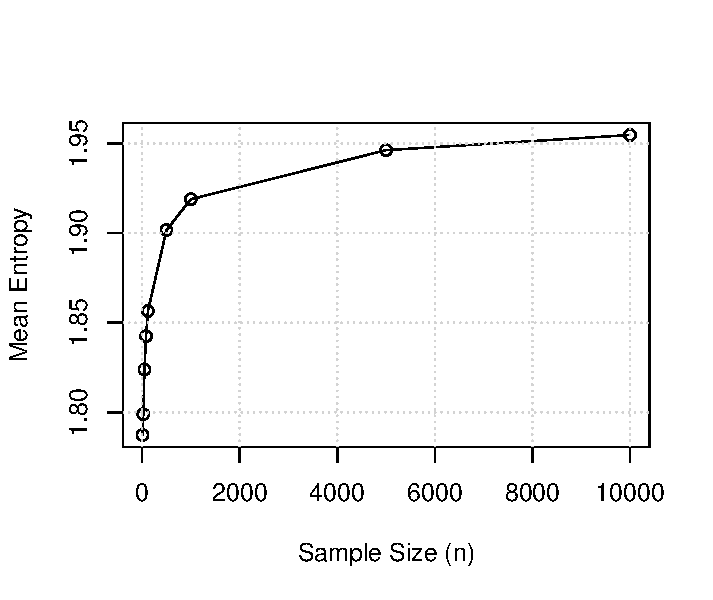
\includegraphics[scale=0.5]{../../../Figures/PDF/mean_entropies1}\vspace{-1.5mm} 
	\caption{Convergence of mean non-parametric entropies.}
	\label{F4}
\end{figure}
%\begin{figure}[H] 
%\centering
	%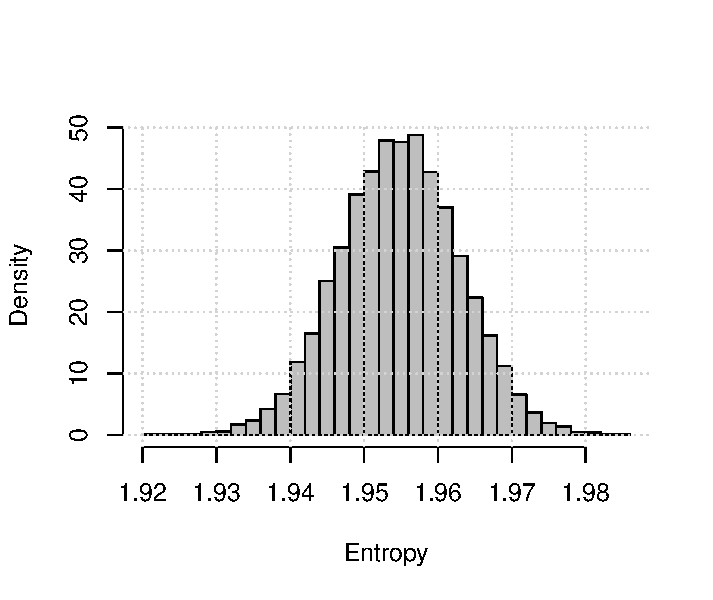
\includegraphics[scale=0.5]{../../../Figures/PDF/histo1}\vspace{-1.5mm} 
	%\caption{Histogram of entropies.}
	%\label{F5}
%\end{figure}
\section{Conclusion}\label{sec_09}

In this article, 

\bibliographystyle{IEEEtran}
%\bibliography{strings,refs}

\bibliography{../../Common/references}\end{document}
